\begin{figure}[t]
\centering
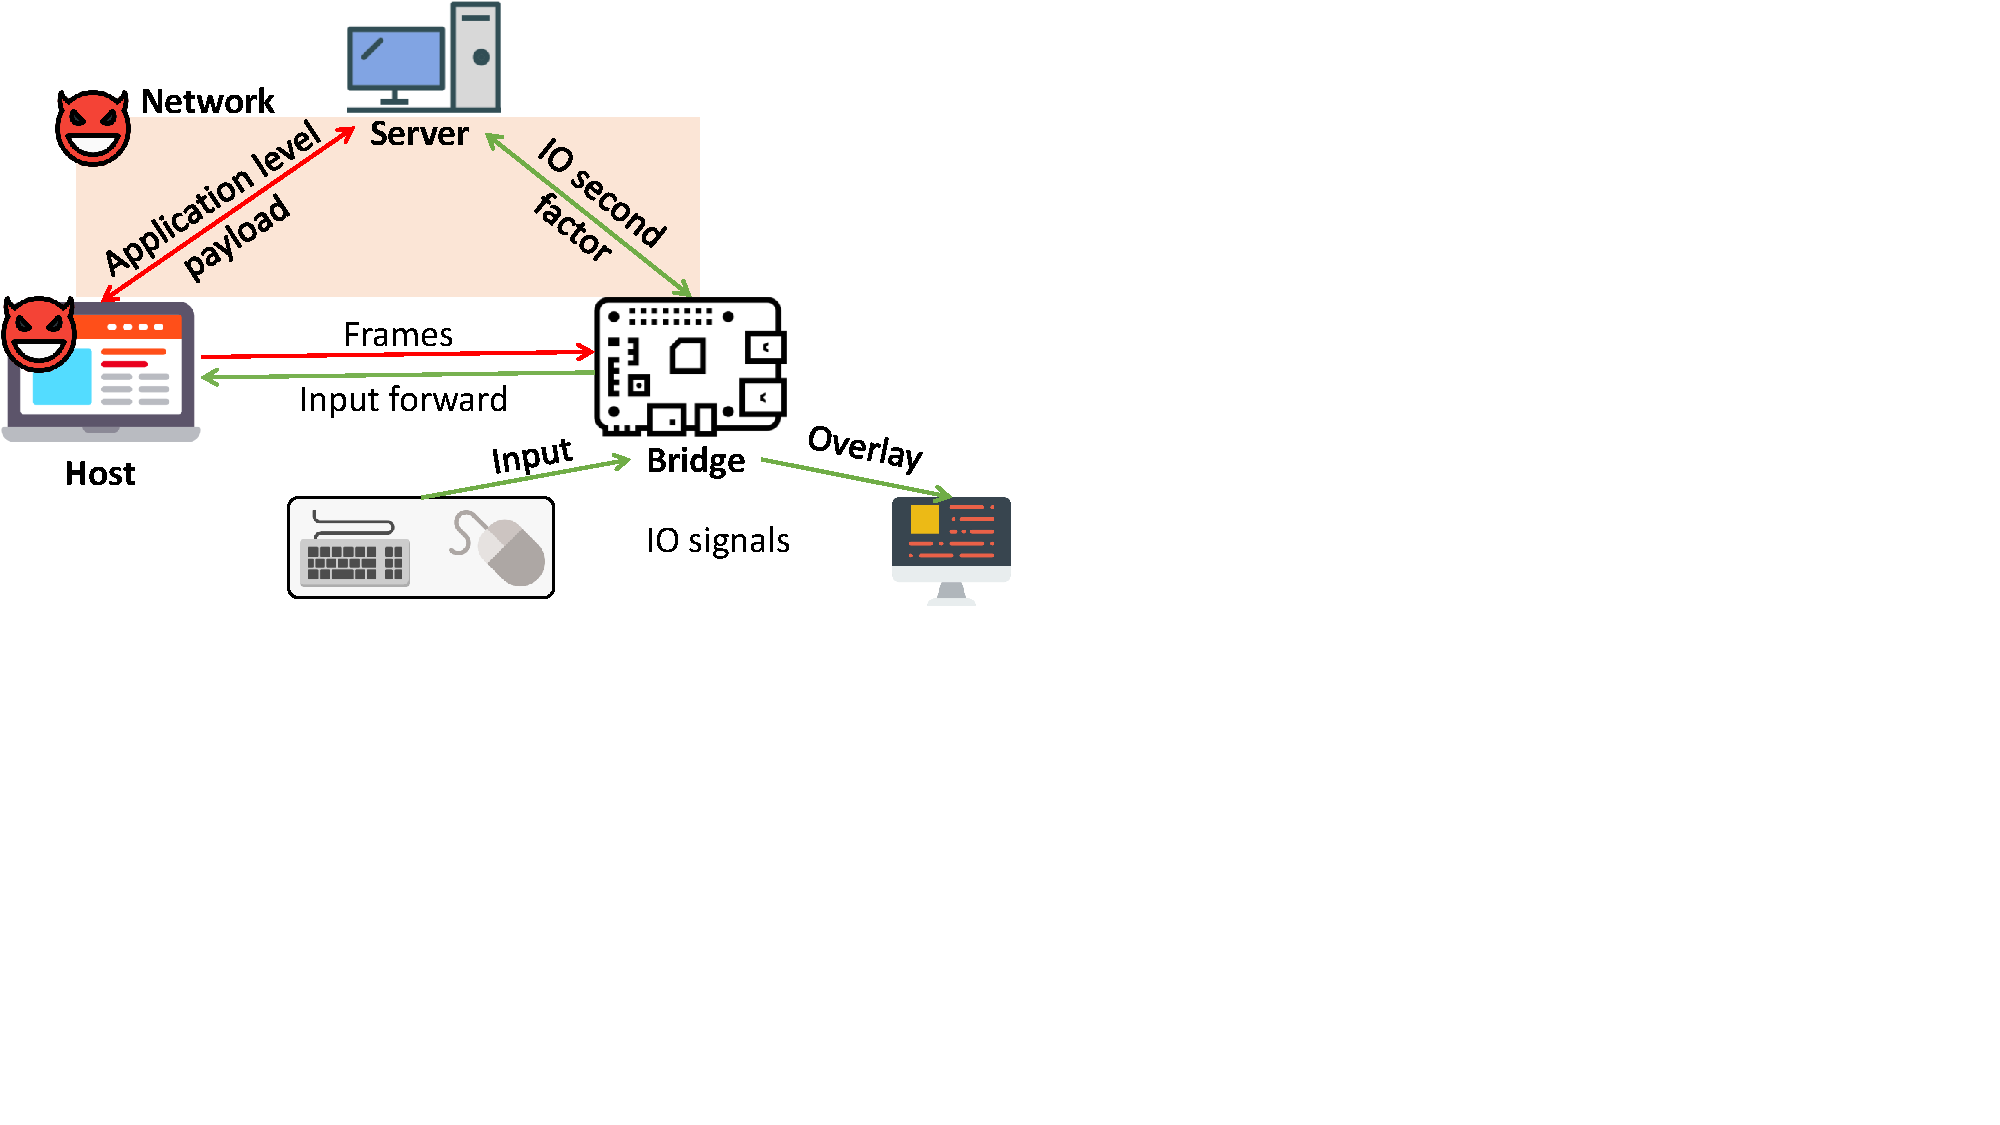
\includegraphics[trim={0 8.5cm 17cm 0}, clip, width=0.85\linewidth]{approachOverview.pdf}
\caption{\textbf{High-level approach overview of our solution.}  The \device connects the trusted IO devices and the attacker-controlled host. 
}
\spacesave
\label{fig:approachOverview}
\centering
\end{figure}

\section{System Overview \& Main Techniques}
\label{sec:approach}

In this section, we present an overview of our solution: \name. On the high-level, \name uses the concept of the \emph{bump in the wire} (such as bump in the ether~\cite{McCPerRei2006}) to provide integrity and confidentiality to the user IO{}s between the IO devices and the remote server. \name achieves this by utilizing a trusted embedded device as a mediator between all the IO devices and the untrusted host. Hence, our approach falls into the category \textbf{B2} (external HW) in Figure~\ref{fig:relatedWorksTree}. 
We call this trusted intermediary \device for the rest of this paper.   


\subsection{System and Attacker Model}
\label{sec:approach:systemAttackerModel}

We consider a system model where the user wants to interact with a trusted remote web server via \red{an attacker-controlled host}. The model is depicted in Figure~\ref{fig:approachOverview} that shows the untrusted host, the remote server, and the user IO devices. We only assume that the monitor, keyboard, mouse (in a word all the IO devices that we need to protect from the malicious host) and the \device are trusted. The \device works as a mediator between all the IO devices and the host. Note that the \device has no network capability to communicate with the server directly, rather it relies on the host and uses it as an untrusted transport. We also assume that the \device comes with preloaded certificates and keys that allow the \device to verify the signatures signed by the server and sign data such as the user input.

There are many possible ways to deploy \name. One way is to assume that the \device manufacturer issues a certificate for each of the deployed \device{}s . The \device maintains a whitelist for the remote servers along with their public certificates. This allows the \device to verify messages signed by those remote servers. Another assumption could be that the \device is issued by a service provider who also runs the remote server. 

\myparagraph{Attacker model and capabilities} Our attacker model assumes that the host (OS, installed applications, and hardware) and the network are attacker-controlled. The attacker can intercept, and arbitrarily manipulate (such as create, drop, or modify) the user IO data between the user and the remote server. 



\subsection{High-level Description of the System}

\begin{figure}[t]
\centering
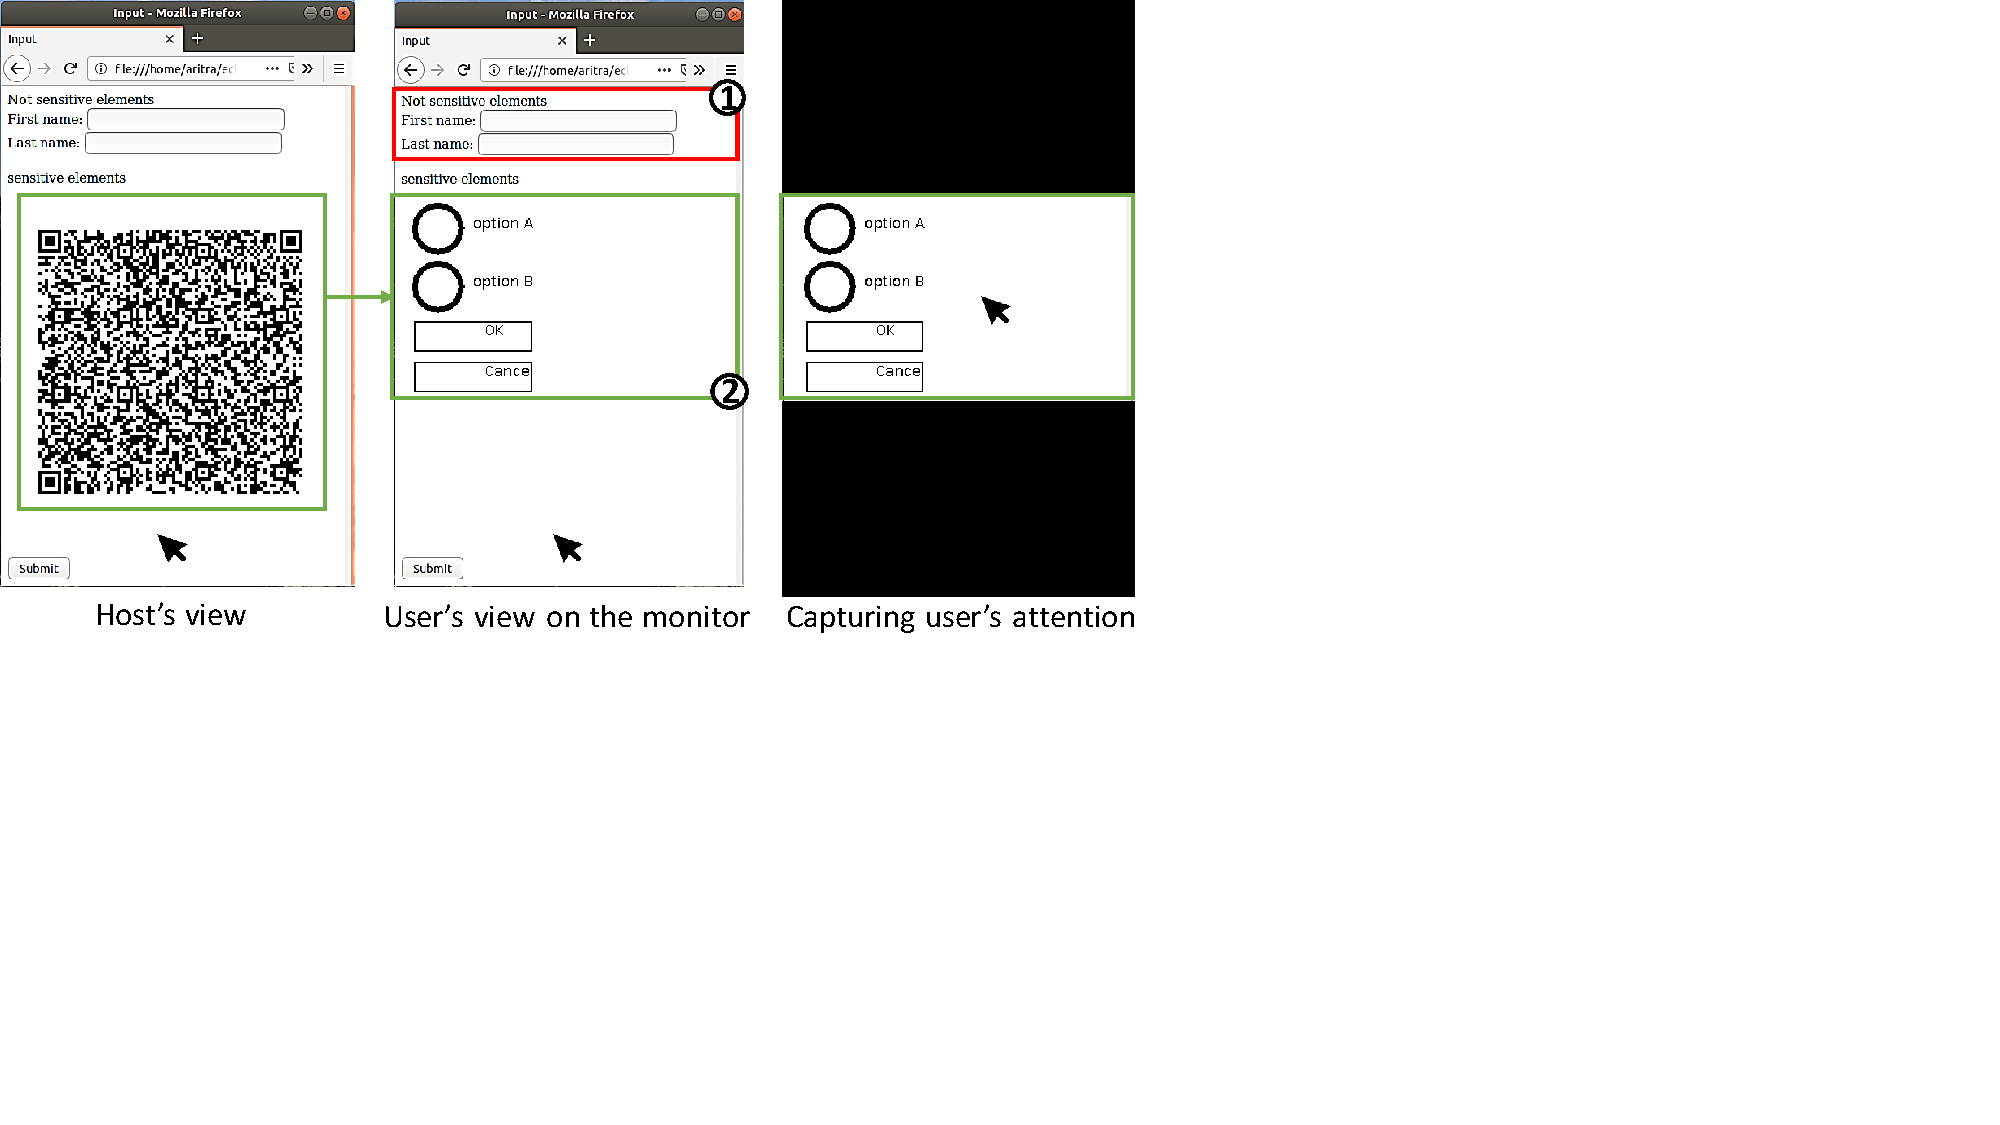
\includegraphics[trim={0 8cm 15cm 0}, clip, width=\linewidth]{overlayScreenShot_new.pdf}
\caption{\textbf{\name's high-level approach} shows that the \device generates UI overlay to protect IO integrity and confidentiality. a) The attacker only sees the non-protected UI elements, and the protected form is encrypted and encoded (in our case, the \device could decode a QR code and decrypt). b) shows the \device generated form overlay that is hidden from the host. The protected part of the screen provides integrity and confidentiality of all user IO. c) shows that the \device dims out (lightbox) the rest of the screen when the user moves her mouse pointer over the protected region to focus user attention.}
\spacesave
\label{fig:screenshot_1}
\end{figure}

\name is build upon the required security and functional properties that are described in Section~\ref{sec:problemStatement:goals}. \name achieves IO integrity \red{and confidentiality} by leveraging an external trusted component that we call \device (refer to Figure~\ref{fig:approachOverview}). 
%In our implementation, \device is realized as an external, low-TCB hardware that uses off-the-shelf components and \device is easy to integrate with legacy systems - providing \emph{easy deployment}. Figure~\ref{fig:approachOverview} illustrates the system configuration. \device sits between IO peripherals and the host system. It intercepts all keyboard and mouse events. Also, it can intercept \& overlay on the display signal. 

\device is active only when the user visits sensitive web applications that require \name security.
Initially, the remote server signs and delivers the sensitive UI elements to the host in a format that is understandable by \device. Next, the host transfers the sensitive UI to \device, and the \device verifies the signature to prevent manipulations by the host. As seen in a running example depicted in Figure~\ref{fig:screenshot_1}, the \device then renders the UI with sensitive elements into an overlay on top of the HDMI frame received from the host. Note that the host cannot access or modify the overlay generated by the \device. Also, the overlay covers only a part of the screen, allowing the other feature-rich content on the webpage to run unmodified. Therefore, this ensures that sensitive UI elements are presented to the user as expected by the remote server -- \emph{output integrity}. For the overlay, we use QR-codes to transfer data from the host to the device because we avoid using extra software/hardware for a separate channel, and it is easy to visualize.

When the user interacts (types or moves the pointer) with the overlay, \device does not forward any event from the keyboard or the mouse to the host. The interaction is maintained solely by \device, which renders on-screen user inputs and therefore offers a user experience that is identical to a typical one as if the \device is not present. The user click on the \emph{submit} button triggers the submission procedure, which consists of the \device signing the user inputs and sending to the server. Note that the text fields of the form and the \emph{submit} button are inside the overlay which is inaccessible by the host, hence the attacker cannot execute the early form submission or clickjacking attacks. Finally, the server verifies the signature of \device to guarantee that the host has not altered the data. Therefore, the \device ensures \emph{input integrity} for all \emph{modalities} of input.


For integrity protection, \name uses well-known user attention focusing mechanisms. Unlike systems like Fidelius, these mechanisms do not introduce any cognitive load to the users due to absence of multiple security indicators.  This allows the user to correctly recognize the overlaid part of the screen that is protected by the system. Thus, the untrusted host cannot trick the user into following malicious instructions when the user interacts with sensitive UI elements. Also, the host cannot observe sensitive data on the overlay because it does not have access to it. 

%Note that the lightbox technique is not the only way to capture the \emph{user attention}, e.g., freezing the untrusted part of the screen is another approach~\cite{huang2012clickjacking}. 
%To minimize user habituation and actively inform the user about the protected overlay, \device activates the user attention mechanism (the lightbox) automatically when the mouse pointer is over the overlay, or the user starts typing to a sensitive text field.
In the case where confidentiality is required, the user manually triggers the lightbox by pressing specific keys. 
